\begin{toreview}

    \subsection{Quantitative Overview of the Field}\label{subsec:results_quantitative}
    % -----------------------------------------------------------------------

    The distribution of the selected literature across the seven concept-matrix categories is illustrated in Figure~\ref{fig:distribution_topics}. Raw article counts alone conflate two different questions: how much a topic is written about, and how dangerous a topic is. A category can dominate the literature because it is easy to publish on, not because it carries the greatest risk. To separate these two questions, we assign each category a \emph{severity score} and compare its rank against its \emph{coverage rank} (article count).

    \subsubsection{Severity Scoring Method}

    The four scoring dimensions are adapted from the "key risks" assessment criteria used in IPCC Working Group II reports, first formalized by Smith et al. \cite{smith2009assessing} and later refined by Oppenheimer et al. \cite{oppenheimer2014emergent} and O'Neill et al. \cite{oneill2017ipcc}, who evaluate climate risks along magnitude, timing, persistence/irreversibility, distributional scope, and likelihood/confidence. We retain the four criteria most transferable to AI risk categories --- magnitude, certainty, irreversibility, and scope --- and drop timing and adaptive-capacity, which are climate-specific. This four-dimension structure also echoes the magnitude/scope/irreversibility triad used in existential risk assessment by Bostrom \cite{bostrom2013existential}, giving the framework precedent within both the climate-risk and AI-safety literatures.

    \begin{itemize}
        \item \textbf{Magnitude (M)}: ceiling of harm if the failure mode materializes (e.g.\ the Treacherous Turn, \cite{bostrom2014superintelligence}).
        \item \textbf{Certainty (C)}: extent of current empirical evidence, as opposed to purely theoretical risk.
        \item \textbf{Irreversibility (I)}: whether the harm is correctable after the fact.
        \item \textbf{Scope (S)}: breadth of population or systems exposed.
    \end{itemize}

    Five independent raters (domain experts) score each category on all four dimensions. The full matrix of raw scores provided by all five raters is available in the Appendix (Table~\ref{tab:rater_scores}). Inter-rater agreement is reported via Krippendorff's $\alpha$ \cite{krippendorff2018content, hayes2007answering}:

    \begin{enumerate}
        \item \alpha = 1 \to perfect agreement
        \item \alpha = 0 \to agreement no better than chance
        \item \alpha < 0 \to systematic disagreement, worse than random
    \end{enumerate}
    
    \subsubsection{Scope Definition for Raters}

    Before scoring, all raters were given the following written scope, to ensure severity judgments reference a common referent rather than each rater's private notion of ``AI'':
        
    \begin{quote}
    \textbf{Scope of ``AI'' for this severity assessment.} Assess the potential harm of each category by considering both:

    \begin{enumerate}
        \item \textbf{Deployed and near-term systems}: current and near-future AI systems (roughly the next 0--3 years), including LLMs and other machine learning systems already in use. Base the assessment on documented incidents or failures that are reasonably likely given existing evidence and literature.

        \item \textbf{Frontier and projected systems}: AI systems that could plausibly emerge through continued improvements to current approaches (roughly a 3 to 15 year horizon, including AGI-adjacent capabilities). Base the assessment on technically grounded failure modes discussed in the research literature, such as deceptive alignment, mesa-optimization, and treacherous turns.
    \end{enumerate}

    Do not consider purely speculative or fictional scenarios that lack support in the current technical literature, such as generic science-fiction robot uprisings. When a category applies to both near-term and frontier systems (as is often the case for \emph{Alignment}), consider both perspectives when assigning its severity.
    \end{quote}

    \begin{table}[h]
        \centering
        \small
        \caption{Mean severity dimension scores across 5 raters. The final row presents ordinal Krippendorff's $\alpha$ to measure inter-rater reliability for each dimension.}
        \label{tab:rater_scores_summary}
        \begin{tabular}{|l|c|c|c|c|}
            \hline
            \textbf{Category} & \textbf{M} & \textbf{C} & \textbf{I} & \textbf{S} \\
            \hline
            Alignment                         & 4.2 & 3.6 & 3.6 & 3.4 \\
            Auditing, Safety \& Oversight     & 3.6 & 4.2 & 3.4 & 3.0 \\
            Human \& Societal Impacts         & 4.2 & 3.8 & 3.8 & 4.6 \\
            Governance, Regulation \& Policy  & 4.2 & 3.6 & 3.8 & 4.0 \\
            Liability \& Ethics               & 3.8 & 3.4 & 2.2 & 2.8 \\
            Explainability / Interpretability & 3.0 & 3.4 & 2.4 & 3.4 \\
            Bias \& Fairness                  & 3.0 & 4.0 & 3.2 & 3.4 \\
            \hline \hline
            \textit{Krippendorff's $\alpha$}  & 0.027 & $-0.113$ & 0.048 & 0.122 \\
            \hline
        \end{tabular}
    \end{table}

    Inter-rater reliability (IRR) was evaluated by calculating ordinal Krippendorff's $\alpha$ for each severity dimension across the seven categories. As presented in the final row of Table~\ref{tab:rater_scores_summary}, agreement across all four dimensions was near zero, well below the standard $\sim$0.67 threshold for acceptable agreement. Given this lack of consensus, and the low number of raters ($n=5$), the severity scores that follow should be treated as indicative rather than definitive; they summarize the raters' central tendency but do not reflect a shared understanding of relative risk across the seven categories.

    \subsubsection{Severity and Coverage}

    Table~\ref{tab:severity_coverage} compares weighted severity scores with the number of papers assigned to each category.

    \begin{table}[h]
        \centering
        \caption{Category severity and literature coverage.}
        \label{tab:severity_coverage}
        \begin{tabular}{|l|c|c|}
            \hline
            \textbf{Category} & \textbf{Severity} & \textbf{Papers} \\
            \hline
            Human \& Societal Impacts         & 4.04 & 35 \\
            Governance, Regulation \& Policy  & 3.92 & 28 \\
            Alignment                         & 3.82 & 29 \\
            Auditing, Safety \& Oversight     & 3.68 & 20 \\
            Bias \& Fairness                  & 3.38 & 8  \\
            Liability \& Ethics               & 3.26 & 8  \\
            Explainability / Interpretability & 3.04 & 12 \\
            \hline
        \end{tabular}
    \end{table}

    Severity and literature coverage do not align perfectly. \emph{Explainability / Interpretability} has the lowest severity score but 12 papers, while \emph{Bias \& Fairness} and \emph{Liability \& Ethics} have higher severity scores but only 8 papers each. \emph{Governance, Regulation \& Policy} also ranks second in severity while having fewer papers than \emph{Alignment}. Overall, research attention broadly follows assessed severity, but some categories receive relatively more or less attention than their severity would suggest.

    % To keep this I would need a citation
    % The relationship between severity and literature coverage can be assessed using Spearman's rank correlation. Using the severity and coverage ranks, the squared rank differences sum to $\sum d_i^2 = 6$. With seven categories, this gives
    % \[
    % \rho = 1 - \frac{6\sum d_i^2}{n(n^2-1)}
    %     = 1 - \frac{6(6)}{7(7^2-1)}
    %     = 0.893.
    % \]
    % This indicates a strong positive association between severity and research coverage: categories ranked as more severe generally receive more research attention. Given the small number of categories ($n=7$), this result should be interpreted cautiously.

	\begin{figure}[htbp]
		\centering
		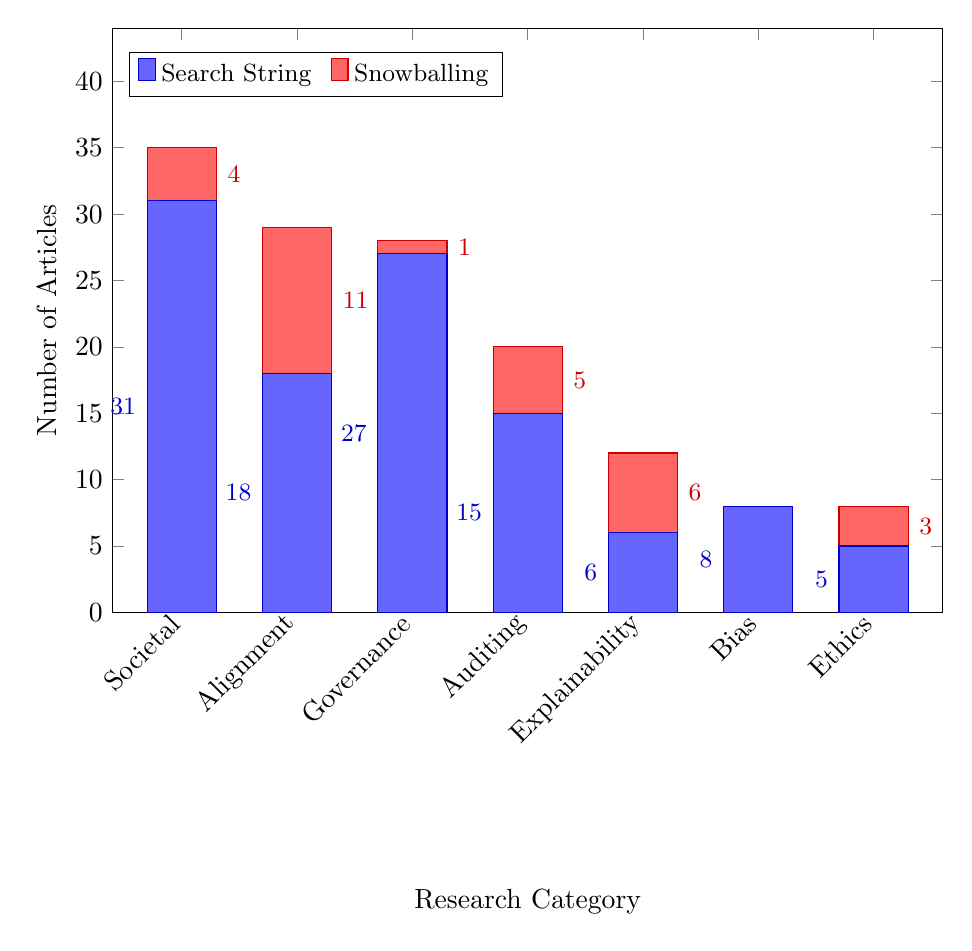
\begin{tikzpicture}
		\begin{axis}[
			ybar stacked,
			symbolic x coords={Societal, Alignment, Governance, Auditing, Explainability, Bias, Ethics},
			xtick=data,
			x tick label style={rotate=45, anchor=east},
			ylabel={Number of Articles},
			xlabel={Research Category},
			xlabel style={yshift=-1.5cm},
			width=\textwidth,
			height=9cm,
			bar width=25pt,
			ymin=0,
			ymax=44,
			legend style={
				at={(0.02,0.96)},
				anchor=north west,
				legend columns=-1,
				font=\small,
				/tikz/every even column/.append style={column sep=5pt}
			}
		]

		% Plot 1: Search String (bottom, BLUE) — label to the LEFT
		\addplot [
			fill=blue!60,
			draw=blue!80!black,
			nodes near coords,
			every node near coord/.style={
				color=blue!80!black,
				font=\small,
				anchor=east,
				xshift=-13pt,
			},
		] coordinates {
			(Societal,31) (Alignment,18) (Governance,27)
			(Auditing,15) (Explainability,6) (Bias,8) (Ethics,5)
		};

		% Plot 2: Snowballing (top, RED) — label to the RIGHT, zeros hidden
		\addplot [
			fill=red!60,
			draw=red!80!black,
			nodes near coords,
			every node near coord/.style={
				color=red!80!black,
				font=\small,
				anchor=west,
				xshift=13pt,
			},
			point meta=explicit symbolic,
		] coordinates {
			(Societal,4)       [4]
			(Alignment,11)     [11]
			(Governance,1)     [1]
			(Auditing,5)       [5]
			(Explainability,6) [6]
			(Bias,0)           [0]
			(Ethics,3)         [3]
		};

		% Plot 3: Invisible — bold black totals above each bar
		\addplot [
			draw=none, fill=none,
			forget plot,
			nodes near coords,
			every node near coord/.style={
				anchor=south,
				yshift=3pt,
				font=\small\bfseries,
				color=black,
			},
			point meta=explicit symbolic,
		] coordinates {
			(Societal,0)       [35]
			(Alignment,0)      [29]
			(Governance,0)     [28]
			(Auditing,0)       [20]
			(Explainability,0) [12]
			(Bias,0)           [8]
			(Ethics,0)         [8]
		};

		\legend{Search String, Snowballing}
		\end{axis}
		\end{tikzpicture}
		\caption{Distribution of research topics across the analyzed literature.}
		\label{fig:distribution_topics}
	\end{figure}

    \vspace{1.5em}

\end{toreview}